\documentclass[11pt]{amsart}

\usepackage[T1]{fontenc}
\usepackage{lmodern}
\usepackage{amssymb,amsmath}
\usepackage{booktabs,array}
\usepackage{graphicx}
\usepackage{tikz}
\usepackage[dvipsnames]{xcolor}
\usepackage[margin=1.15in]{geometry}
\usepackage[colorlinks=true,linkcolor=blue!50!black,citecolor=blue!50!black,urlcolor=blue!50!black]{hyperref}

\newtheorem{theorem}{Theorem}[section]
\newtheorem{proposition}[theorem]{Proposition}
\newtheorem{lemma}[theorem]{Lemma}
\newtheorem{corollary}[theorem]{Corollary}
\theoremstyle{definition}
\newtheorem{definition}[theorem]{Definition}
\newtheorem{innerconj}{Conjecture}
\newenvironment{conjecture}[1]{\renewcommand{\theinnerconj}{#1}\innerconj}{\endinnerconj}
\theoremstyle{remark}
\newtheorem{remark}[theorem]{Remark}

\numberwithin{equation}{section}

\newcommand{\GP}{\mathrm{GP}}
\hypersetup{pdftitle={The parity conjecture for independence polynomials of generalized Petersen graphs contradicts itself},pdfauthor={Deep Bhattacharjee}}
\providecommand{\doi}[1]{\url{https://doi.org/#1}}

\begin{document}

\title[Independence polynomials of generalized Petersen graphs]{The parity conjecture for independence polynomials\\ of generalized Petersen graphs contradicts itself}

\author{Deep Bhattacharjee}
\address{Formerly, Electro-Gravitational Space Propulsion Laboratory (EGSPL),\newline Bhubaneswar, Odisha 751030, India}
\email{d.bhattacharjee@erl-forschung.de}
\email{itsdeep@live.com}
\urladdr{https://orcid.org/0000-0003-0466-750X}
\thanks{Corresponding author: \href{mailto:d.bhattacharjee@erl-forschung.de}{d.bhattacharjee@erl-forschung.de}; ORCID \href{https://orcid.org/0000-0003-0466-750X}{\mbox{0000-0003-0466-750X}}}

\subjclass[2020]{Primary 05C31; Secondary 05C60, 26C10}
\keywords{independence polynomial, real roots, generalized Petersen graph, graph isomorphism}

\begin{abstract}
Pandey conjectured that for $n\ge 2k+1$ the independence polynomial of the generalized Petersen graph $\GP(n,k)$ has only real roots if and only if $k$ is even. Erlbacher's Demonstrandum project refuted this by exact computation, with $\GP(7,3)$, $\GP(9,2)$ and the isomorphism $\GP(7,2)\cong\GP(7,3)$. We show that the statement contradicts itself for every $n\equiv 3\pmod 4$, since then $\GP(n,2)\cong\GP(n,(n-1)/2)$ and $(n-1)/2$ is odd, and we give short proofs that each direction fails on its own.
\end{abstract}

\maketitle

\section{Introduction}

For integers $n\ge3$ and $1\le k<n/2$, the generalized Petersen graph $\GP(n,k)$ of Watkins~\cite{Watkins} has vertices $u_0,\dots,u_{n-1}$ and $v_0,\dots,v_{n-1}$ and the edges
\[
u_iu_{i+1},\qquad u_iv_i,\qquad v_iv_{i+k}\qquad(0\le i<n),
\]
with indices read modulo $n$. The independence polynomial of a graph $G$ is $I(G;x)=\sum_{j\ge0}a_jx^j$, where $a_j$ is the number of independent sets of $G$ with $j$ vertices; its roots are always real for some families and spread over the plane for others~\cite{BHN}. Real-rootedness of independence polynomials is known for claw-free graphs by the theorem of Chudnovsky and Seymour~\cite{CS}; generalized Petersen graphs are cubic and contain claws, and their roots were studied numerically by Pandey~\cite{Pandey}, who proposed the following.

\begin{conjecture}{4.1 of \cite{Pandey}}\label{conj}
For all integers $n\ge 2k+1$, the polynomial $I(\GP(n,k);x)$ has only real roots if and only if $k$ is even.
\end{conjecture}

The conjecture assigns a property to the pair $(n,k)$, whereas real-rootedness depends only on the isomorphism class of $\GP(n,k)$. Different step sizes can give the same graph, and this is enough to refute it.

\begin{theorem}\label{thm:main}
The following hold.
\begin{enumerate}
\item[(a)] If $n\equiv 3\pmod 4$ and $n\ge 7$, then $\GP(n,2)\cong\GP(n,\tfrac{n-1}2)$, the step $\tfrac{n-1}2$ is odd, and both pairs $(n,2)$ and $(n,\tfrac{n-1}2)$ satisfy $n\ge 2k+1$. So Conjecture~\ref{conj} fails for at least one of these two pairs, for every such $n$.
\item[(b)] $I(\GP(7,3);x)$ has only real roots, although $3$ is odd.
\item[(c)] $I(\GP(9,2);x)$ has exactly five real roots and one pair of non-real roots, although $2$ is even.
\end{enumerate}
\end{theorem}

Part~(a) is a statement about isomorphisms alone and needs no knowledge of the polynomials. Parts~(b) and~(c) show that neither implication of the conjecture survives separately.

The conjecture was first refuted by the Demonstrandum project of Erlbacher~\cite{Dem}, which computed the polynomials of $\GP(7,3)$ and $\GP(9,2)$ exactly, counted their real roots with Sturm sequences, and noted the isomorphism $\GP(7,2)\cong\GP(7,3)$; it also noted that the triangular prism $\GP(3,1)$, whose polynomial is $1+6x+6x^2$, is real-rooted. Parts~(b) and~(c) are therefore theirs, and we include them with proofs that need only sign changes and Vieta's formulas. Part~(a) turns their isomorphism into an infinite family.

\section{Isomorphic generalized Petersen graphs}

\begin{lemma}\label{lem:iso}
Let $1\le k,l<n/2$ with $kl\equiv\pm1\pmod n$. Then the map $\varphi(u_i)=v_{li}$, $\varphi(v_i)=u_{li}$ is an isomorphism from $\GP(n,k)$ onto $\GP(n,l)$.
\end{lemma}

\begin{proof}
Since $kl\equiv\pm1$, the number $l$ is invertible modulo $n$, so $i\mapsto li$ permutes the indices and $\varphi$ is a bijection. It maps the outer edge $u_iu_{i+1}$ to $v_{li}v_{li+l}$, an inner edge of $\GP(n,l)$; the spoke $u_iv_i$ to the spoke $v_{li}u_{li}$; and the inner edge $v_iv_{i+k}$ to $u_{li}u_{li+lk}=u_{li}u_{li\pm1}$, an outer edge. Both graphs have $3n$ edges, so $\varphi$ is an isomorphism.
\end{proof}

\begin{figure}[t]
\centering
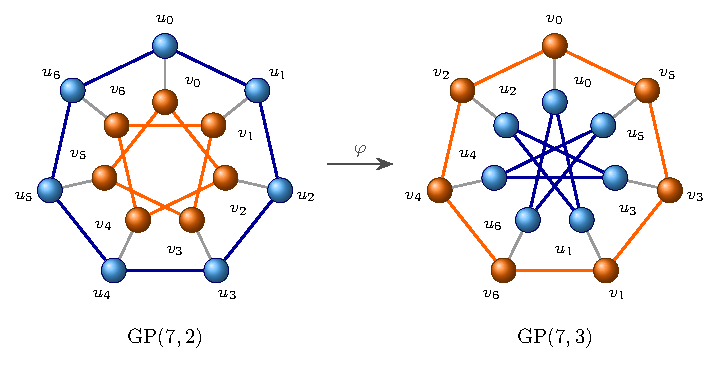
\includegraphics[width=0.92\textwidth]{figures/gp7}
\caption{The isomorphism $\varphi$ of Lemma~\ref{lem:iso} for $n=7$, $k=2$, $l=3$. Each vertex of $\GP(7,3)$ carries the name of its preimage. The outer cycle of $\GP(7,2)$ (blue) becomes the inner cycle of $\GP(7,3)$, and the inner cycle (orange) becomes the outer one.}
\label{fig:gp7}
\end{figure}

Steimle and Staton~\cite{SS} proved that these maps, together with $\GP(n,k)=\GP(n,n-k)$, account for all isomorphisms between generalized Petersen graphs; we only need the easy direction above.

\begin{proof}[Proof of Theorem~\ref{thm:main}(a)]
Let $n\equiv3\pmod 4$, $n\ge7$, and $l=(n-1)/2$. Then $2l=n-1\equiv-1\pmod n$, so $\GP(n,2)\cong\GP(n,l)$ by Lemma~\ref{lem:iso}. Since $n-1\equiv 2\pmod 4$, $l$ is odd, and $n=2l+1\ge 2\cdot2+1$. Conjecture~\ref{conj} for $(n,2)$ says that $I(\GP(n,2);x)$ is real-rooted, and for $(n,l)$ that the same polynomial is not.
\end{proof}

The same argument applies whenever some even $k$ and odd $l$ below $n/2$ satisfy $kl\equiv\pm1\pmod n$; for instance $4\cdot3\equiv-1\pmod{13}$ gives $\GP(13,4)\cong\GP(13,3)$.

\section{The two polynomials}

Counting independent sets of each size gives
\begin{align}
I(\GP(7,2);x)&=1+14x+70x^2+154x^3+147x^4+49x^5,\label{eq:p7}\\
I(\GP(9,2);x)&=1+18x+126x^2+438x^3+801x^4+747x^5+303x^6+27x^7.\label{eq:p9}
\end{align}
Some coefficients can be read off at once: $a_1$ is the number of vertices and $a_2=\binom{2n}2-3n$, since $\GP(n,k)$ has $3n$ edges. Since $2\cdot 3\equiv-1\pmod 7$, Lemma~\ref{lem:iso} gives $\GP(7,3)\cong\GP(7,2)$, so \eqref{eq:p7} is also the independence polynomial of $\GP(7,3)$ (Figure~\ref{fig:gp7}).

\begin{proof}[Proof of Theorem~\ref{thm:main}(b)]
Let $P$ be the polynomial \eqref{eq:p7}. Its values at seven points are
\[
\renewcommand{\arraystretch}{1.5}
\begin{array}{c*{7}{>{\displaystyle}c}}
\toprule
x & -\frac75 & -\frac{13}{10} & -1 & -\frac35 & -\frac3{10} & -\frac15 & -\frac1{10}\\
P(x) & -\frac{8733}{3125} & \frac{67513}{10^5} & 1 & -\frac{697}{3125} & \frac{1363}{10^5} & -\frac{39}{3125} & \frac{16021}{10^5}\\
\bottomrule
\end{array}
\]
The sign changes five times along the table, so $P$ has a root in each of the five disjoint intervals $(-\frac75,-\frac{13}{10})$, $(-1,-\frac35)$, $(-\frac35,-\frac3{10})$, $(-\frac3{10},-\frac15)$ and $(-\frac15,-\frac1{10})$. As $P$ has degree five, all its roots are real. By the remark above, $P=I(\GP(7,3);x)$, and $3$ is odd.
\end{proof}

\begin{proof}[Proof of Theorem~\ref{thm:main}(c)]
Let $Q$ be the polynomial \eqref{eq:p9}. Its sign at the ten points below changes across each of the five intervals
\[
\begin{gathered}
Q(-8.28862)<0<Q(-8.28861),\qquad Q(-0.51657)>0>Q(-0.51656),\\
Q(-0.31262)<0<Q(-0.31261),\qquad Q(-0.22263)>0>Q(-0.22262),\\
Q(-0.16871)<0<Q(-0.16870),
\end{gathered}
\]
so $Q$ has real roots $\rho_1,\dots,\rho_5$, one in each interval. Let $r$ and $r'$ be the two remaining roots, counted with multiplicity. Since $Q$ has degree seven with leading coefficient $27$, the relations between roots and coefficients give
\[
r+r'=-\frac{303}{27}-\sum_{i=1}^5\rho_i,\qquad rr'=-\frac{1}{27\,\rho_1\rho_2\rho_3\rho_4\rho_5}.
\]
Both numbers are real. Adding the endpoints of the intervals gives $-9.50915<\sum\rho_i<-9.50910$, so $-1.713123<r+r'<-1.713071$ and $(r+r')^2<2.9348$. All $\rho_i$ are negative and $|\rho_1\cdots\rho_5|<8.28862\cdot0.51657\cdot0.31262\cdot0.22263\cdot0.16871<0.050278$, so $rr'>1/(27\cdot0.050278)>0.7366$ and $4rr'>2.9464$. Hence
\[
(r-r')^2=(r+r')^2-4rr'<0,
\]
so $r-r'$ is not real, and $r$ and $r'$ are complex conjugates that are not real. Thus $Q=I(\GP(9,2);x)$ has exactly five real roots, although $2$ is even.
\end{proof}

\begin{remark}
The non-real pair of $I(\GP(9,2);x)$ is close to $-0.85655\pm0.05554\,i$. In~\cite{Pandey} the polynomials were computed with a transfer matrix whose entries carry the weight $x^{|B|}$, where $|B|$ is the number of occupied positions in a state that also records earlier inner vertices; with this weighting a vertex is counted once for every state in which it appears. The report there of $50$ roots for $\GP(25,2)$ reflects this: the spokes $u_iv_i$ cover every vertex and an independent set meets each spoke at most once, so $I(\GP(25,2);x)$ has degree at most $25$. The polynomials behind the numerical evidence in~\cite{Pandey} are therefore not independence polynomials.
\end{remark}

\subsection*{Use of generative AI} The author used Claude (Anthropic) for literature search, computation and drafting; the author checked the mathematics and takes full responsibility for the content.

\begin{thebibliography}{9}

\bibitem{BHN}
J.~I. Brown, C.~A. Hickman and R.~J. Nowakowski, \emph{On the location of roots of independence polynomials}, J. Algebraic Combin. \textbf{19} (2004), 273--282. \doi{10.1023/B:JACO.0000030703.39946.70}

\bibitem{CS}
M.~Chudnovsky and P.~Seymour, \emph{The roots of the independence polynomial of a clawfree graph}, J. Combin. Theory Ser.~B \textbf{97} (2007), 350--357. \doi{10.1016/j.jctb.2006.06.001}

\bibitem{Dem}
J.~Erlbacher, \emph{Demonstrandum verified artifacts: nine papers in combinatorics (counterexamples, records, theorems, and Lean formalizations)}, software and data, 2026, result~6. \doi{10.5281/zenodo.20673864}

\bibitem{Pandey}
R.~Pandey, \emph{Parity-dependent real-rootedness in independence polynomials of generalized Petersen graphs}, preprint, 2026. \href{https://arxiv.org/abs/2601.03293}{arXiv:2601.03293}

\bibitem{SS}
A.~Steimle and W.~Staton, \emph{The isomorphism classes of the generalized Petersen graphs}, Discrete Math. \textbf{309} (2009), 231--237. \doi{10.1016/j.disc.2007.12.074}

\bibitem{Watkins}
M.~E. Watkins, \emph{A theorem on Tait colorings with an application to the generalized Petersen graphs}, J. Combin. Theory \textbf{6} (1969), 152--164. \doi{10.1016/S0021-9800(69)80116-X}

\end{thebibliography}

\end{document}
